\documentclass[a4paper,10pt]{article}
\usepackage{polski}
\usepackage[utf8]{inputenc}
\usepackage{array,floatflt,textcomp,graphicx,longtable}
%custom margins
\usepackage[left=3cm, top=2.5cm, bottom=3cm, right=2cm, foot=2cm, head=0.5cm]{geometry}
\usepackage{fancyhdr}
\usepackage[bookmarks=true, pdftex]{hyperref}

%styl nagłowków
\pagestyle{fancy} 
\parindent 2cm 

%opening
\title{Analiza obiektowa}
\author{3@KASK}

\begin{document}
\bibliographystyle{plain}


\maketitle


\begin{center}
%budowanie tabeli
\begin{longtable}{|p{7cm}|p{7cm}|}
\hline
Symbol projektu: & Opiekun projektu:   \tabularnewline 
3@KASK & mgr inż. Tomasz Boiński    \tabularnewline \hline
\multicolumn{2}{|l|}{Nazwa Projektu: } \tabularnewline
\multicolumn{2}{|l|}{Wizualizacja grafów za pomocą biblioteki Prefuse } \tabularnewline 
\hline
\multicolumn{2}{l}{ } \tabularnewline %pusta linijka
\hline 
Nazwa Dokumentu: & Nr wersji:   \tabularnewline 
Analiza obiektowa & 2.2 \tabularnewline \hline
Odpowiedzialny za dokument: & Data pierwszego sporządzenia:   \tabularnewline 
Piotr Kunowski & 23 maja 2009 \tabularnewline \hline
Przeznaczenie: & Data ostatniej aktualizacji:   \tabularnewline 
DLA KLIENTA & \today \tabularnewline \hline
\end{longtable}
\end{center}


\begin{center}
\begin{longtable}{|c|p{4cm}|c|c|c|}
\multicolumn{5}{c}{\textbf{Historia dokumentu}} \tabularnewline \hline
\textbf{Wersja} & \textbf{Opis modyfikacji} & \textbf{Rozdział/strona} & \textbf{Autor modyfikacji} & \textbf{Data} \tabularnewline \hline 
1 & Stworzenie & wszystkie & Grupa projektowa & 23.05.09 \tabularnewline \hline
1.1 & Dodano pakiet Utils & 1, 3 & Anna Jaworska & 2.06.09 \tabularnewline \hline
2 & Dodano zaktualizowane diagramy oraz opisy klas & wszystkie & Grupa projektowa & 16.06.09 \tabularnewline \hline
2.1 & Aktualizacja pakietu Options & 2 & Radosław Kleczkowski & 12.10.10 \tabularnewline \hline
2.2 & Aktualizacja pozostałych pakietów & 3, 4, 5, 6, 7 & Radosław Kleczkowski & 15.10.10 \tabularnewline \hline

\end{longtable}
\end{center}


\newpage
\tableofcontents
\newpage

\section{Pakiety}

\subsection{Diagram}
 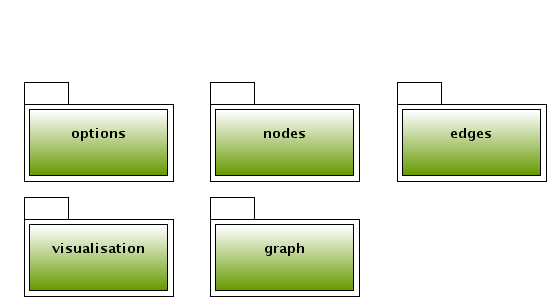
\includegraphics[width=\linewidth]{./modelowanie/OV_UML/PackageDiagram.png}

\newpage
\subsection{Opis pakietów}


\begin{center}
\begin{longtable}{|m{3cm}|m{9cm}|} \hline

P001 & options\\ \hline
Opis: & Pakiet zawierający klasy z polami opisującymi różne (modyfikowalne) ustawienia wizualizacji takie jak: kolory, grubość linii itp.     \\ \hline
Interfejsy: &     \\ \hline
Realizowane wymagania: & WF002, WF001, WI004 \\ \hline
Priorytet: & średnio ważne \\ \hline

\multicolumn{2}{c}{} \\
 \hline

P002 & nodes\\ \hline
Opis: & Pakiet z klasami odpowiedzialnymi za wizualizację i przechowywanie danych o wierzchołkach.    \\ \hline
Interfejsy: &     \\ \hline
Realizowane wymagania: & WF004, WF005, WF006, WF007, WI004 \\ \hline
Priorytet: & bardzo ważne \\ \hline

\multicolumn{2}{c}{} \\
 \hline

P003 & edges\\ \hline
Opis: & Pakiet z klasami odpowiedzialnymi za wizualizację i przechowywanie danych o krawędziach.    \\ \hline
Interfejsy: &     \\ \hline
Realizowane wymagania: & WF006, WF007, WI004 \\ \hline
Priorytet: & bardzo ważne \\ \hline

\multicolumn{2}{c}{} \\
 \hline

P004 & visualization\\ \hline
Opis: & Zawiera dodatkowe klasy przydatne w wizualizacji.\\ \hline
Interfejsy: &     \\ \hline
Realizowane wymagania: & WF001, WF008, WI004 \\ \hline
Priorytet: & średnio ważne \\ \hline

\multicolumn{2}{c}{} \\
 \hline

P005 & graph\\ \hline
Opis: & Pakiet zawiera klasy, które zawierają podstawowe operacje na danych OwlApi oraz graph. \\ \hline
Interfejsy: &     \\ \hline
Realizowane wymagania: & WD001 \\ \hline
Priorytet: & bardzo ważne \\ \hline

%\multicolumn{2}{c}{} \\
% \hline
\multicolumn{2}{c}{} \\
 \hline

P006 & utils\\ \hline
Opis: & Pakiet zawiera klasy pomocnicze \\ \hline
Interfejsy: &     \\ \hline
Realizowane wymagania: & CF005 \\ \hline
Priorytet: & bardzo ważne \\ \hline

\end{longtable}

\end{center}

\section{Pakiet options}

\subsection{Diagram}

 \scalebox{0.3}{ 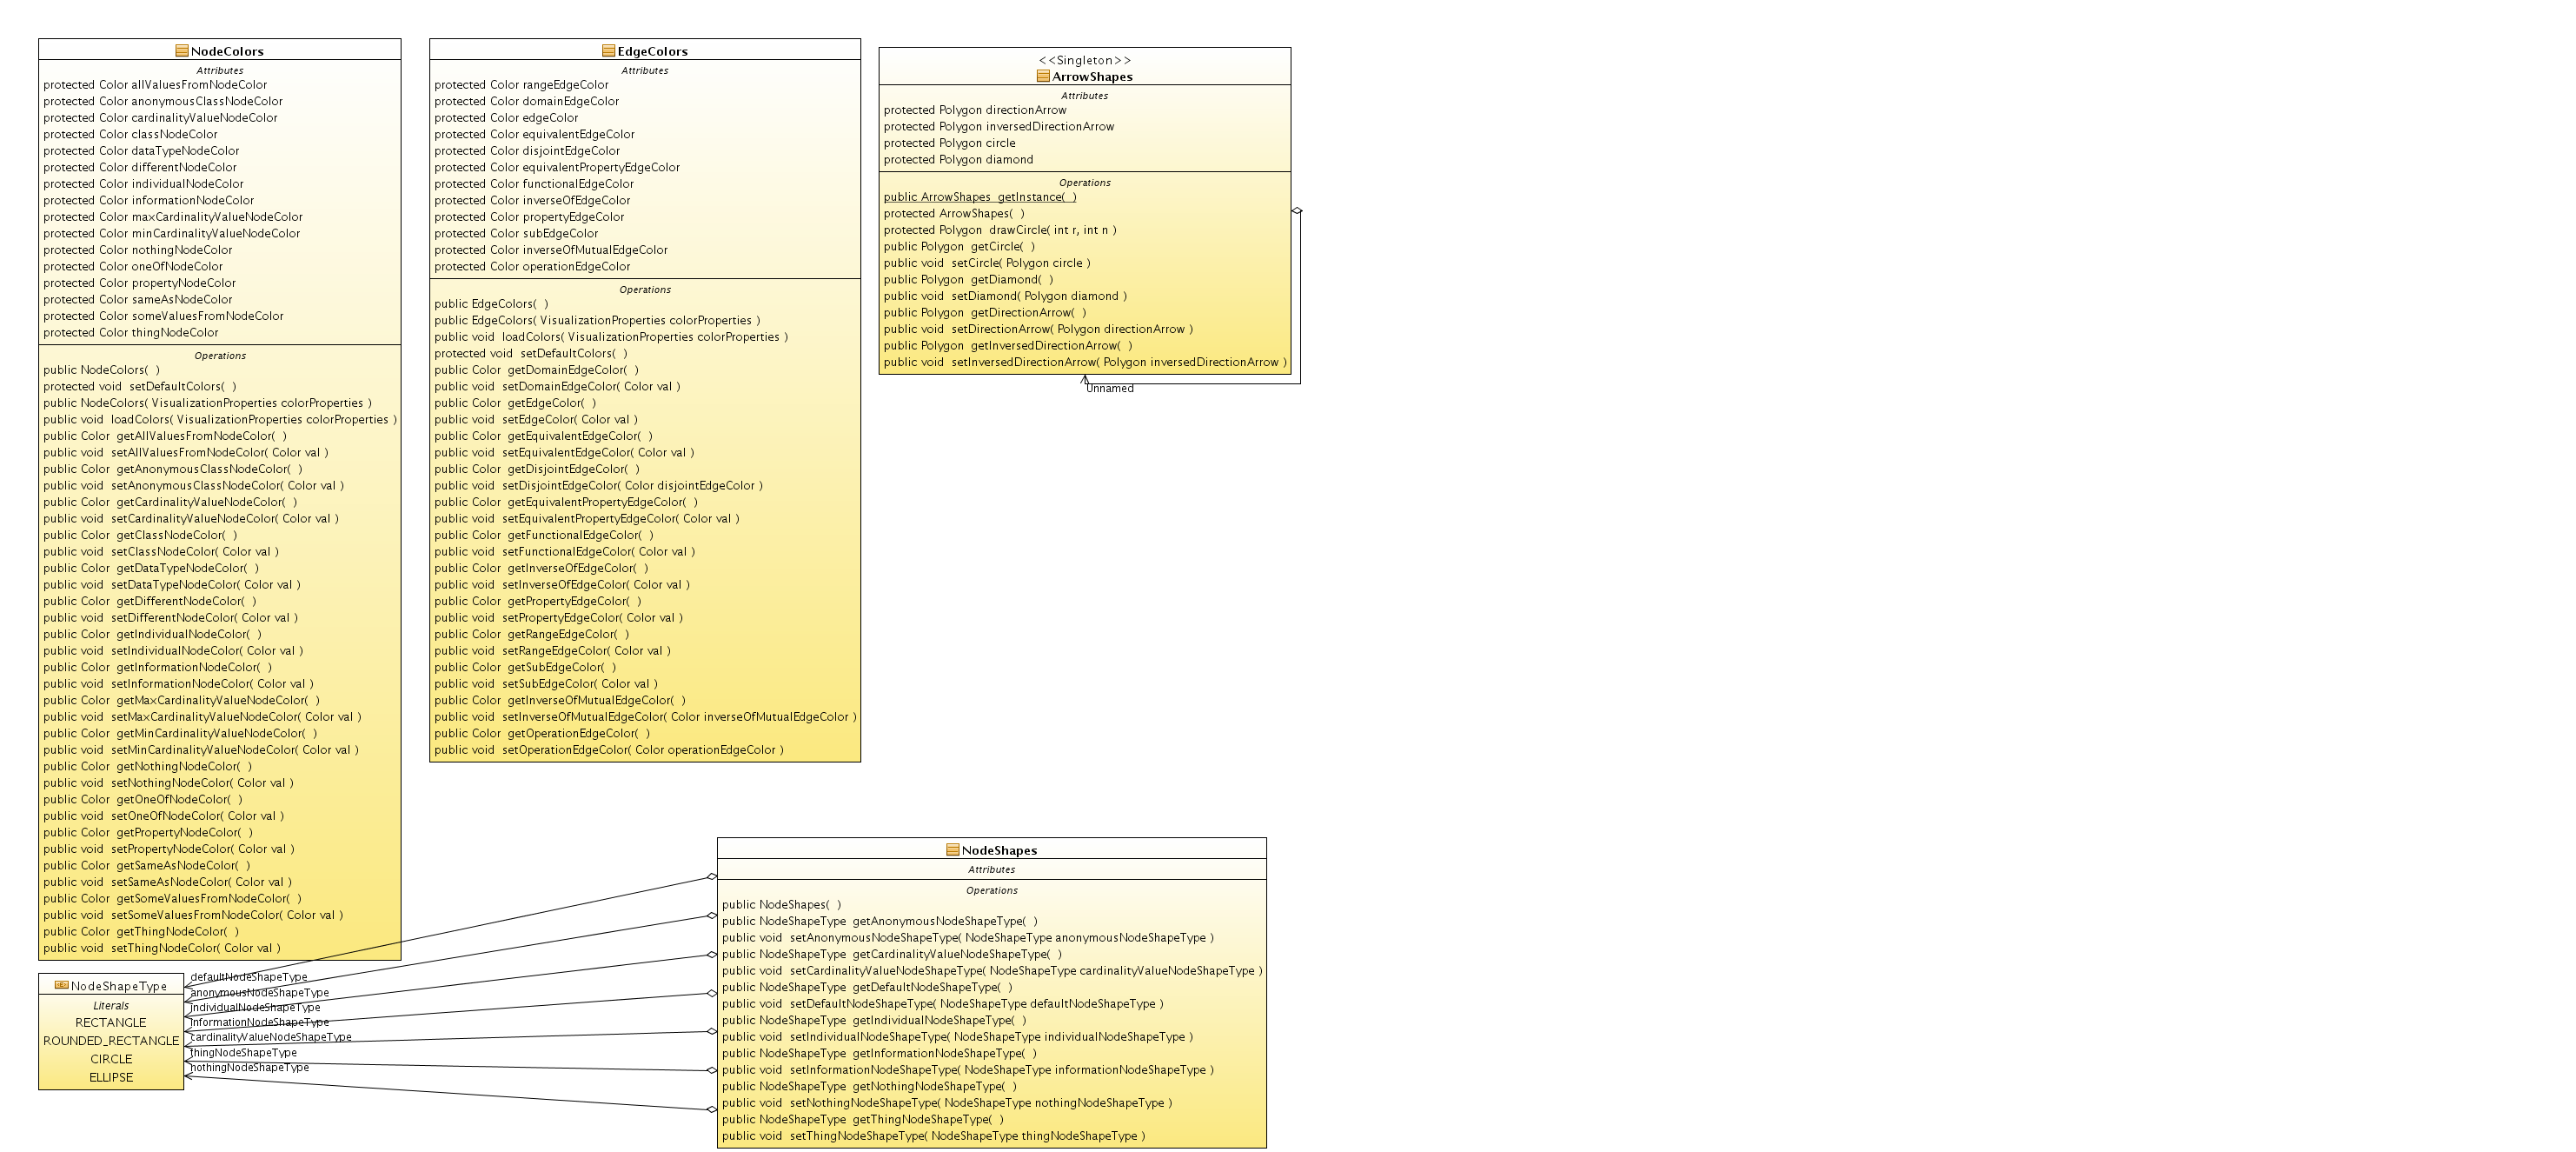
\includegraphics{./modelowanie/OV_UML/OptionsClassDiagram.png}}



\subsection{Opis klasy}

\begin{center}
 


\begin{longtable}{|m{3cm}|m{9cm}|} \hline

CO001 & EdgeColors \\ \hline
Opis: & Zawiera definicje kolorów dla poszczególnych rodzajów krawędzi.   \\ \hline
Klasy nadrzędne: &     \\ \hline
Atrybuty: & \begin{itemize}
 \item domainEdgeColor
 \item edgeColor
 \item equivalentEdgeColor
 \item equivalentPropertyEdgeColor
 \item functionalEdgeColor
 \item inverseOfEdgeColor
 \item propertyEdgeColor
 \item rangeEdgeColor
 \item subEdgeColor

\end{itemize}
 \\ \hline
Metody: & %\begin{itemize}
% \item 
%\end{itemize}
  \\ \hline
Realizowane wymagania: & WF002 \\ \hline
Priorytet: & średnio ważny \\ \hline

\multicolumn{2}{c}{} \\
 \hline

CO002 & NodeColors \\ \hline
Opis: & Zawiera definicje kolorów dla poszczególnych rodzajów krawędzi.   \\ \hline
Klasy nadrzędne: &     \\ \hline
Atrybuty: & \begin{itemize}
 \item allValuesFromNodeColor
 \item cardinalityNodeColor
 \item cardinalityValueNodeColor
 \item classNodeColor
 \item complementOfNodeColor
 \item dataTypeNodeColor
 \item differentNodeColor
 \item functionalPropertyNodeColor
 \item individualNodeColor
 \item informationNodeColor
 \item intersectionOfNodeColor
 \item inverseFunctionalNodeColor
 \item maxCardinalityValueNodeColor
 \item minCardinalityValueNodeColor
 \item nothingNodeColor
 \item oneOfNodeColor
 \item propertyNodeColor
 \item sameAsNodeColor
 \item someValuesFromNodeColor
 \item symmetricPropertNodeColor
 \item thingNodeColor
 \item transitivePropertyNodeColor
 \item unionOfNodeColor 
\end{itemize}
 \\ \hline
Metody: & %\begin{itemize}
 %\item 
%\end{itemize}
  \\ \hline
Realizowane wymagania: & WF002 \\ \hline
Priorytet: & średnio ważny \\ \hline

%\multicolumn{2}{c}{} \\
% \hline


\multicolumn{2}{c}{} \\
 \hline

CO003 & ArrowShapes \\ \hline
Opis: & Singleton przechowujący kształty grotów dla strzałek.   \\ \hline
Klasy nadrzędne: &     \\ \hline
Atrybuty: & \begin{itemize}
 \item directionArrow
 \item inversedDirectionArrow
 \item circle
 \item diamond

\end{itemize}
 \\ \hline
Metody: & %\begin{itemize}
% \item 
%\end{itemize}
  \\ \hline
Realizowane wymagania: & WF002 \\ \hline
Priorytet: & średnio ważny \\ \hline

\multicolumn{2}{c}{} \\
 \hline

CO004 & NodeShapes \\ \hline
Opis: & Klasa przechowująca informacje o kształtach poszczególnych węzłów.   \\ \hline
Klasy nadrzędne: &     \\ \hline
Atrybuty: & \begin{itemize}
 \item defaultNodeShapeType
 \item anonymousNodeShapeType
 \item individualNodeShapeType
 \item informationNodeShapeType
 \item cardinalityValueNodeShapeType
 \item thingNodeShapeType
 \item NodeShapeType nothingNodeShapeType

\end{itemize}
 \\ \hline
Metody: & %\begin{itemize}
% \item 
%\end{itemize}
  \\ \hline
Realizowane wymagania: & WF002 \\ \hline
Priorytet: & średnio ważny \\ \hline

\multicolumn{2}{c}{} \\
 \hline

CO005 & NodeShapeType \\ \hline
Opis: &  Enum - rodzaje kształtów dla węzłów grafu.   \\ \hline
Klasy nadrzędne: &     \\ \hline
Atrybuty: & \begin{itemize}
 \item RECTANGLE
 \item ROUNDED\_RECTANGLE
 \item CIRCLE
 \item ELLIPSE

\end{itemize}
 \\ \hline
Metody: & %\begin{itemize}
% \item 
%\end{itemize}
  \\ \hline
Realizowane wymagania: & WF002 \\ \hline
Priorytet: & średnio ważny \\ \hline


\end{longtable}
\end{center}

\section{Pakiet nodes}

\subsection{Diagram}

\begin{center}
\scalebox{0.57}{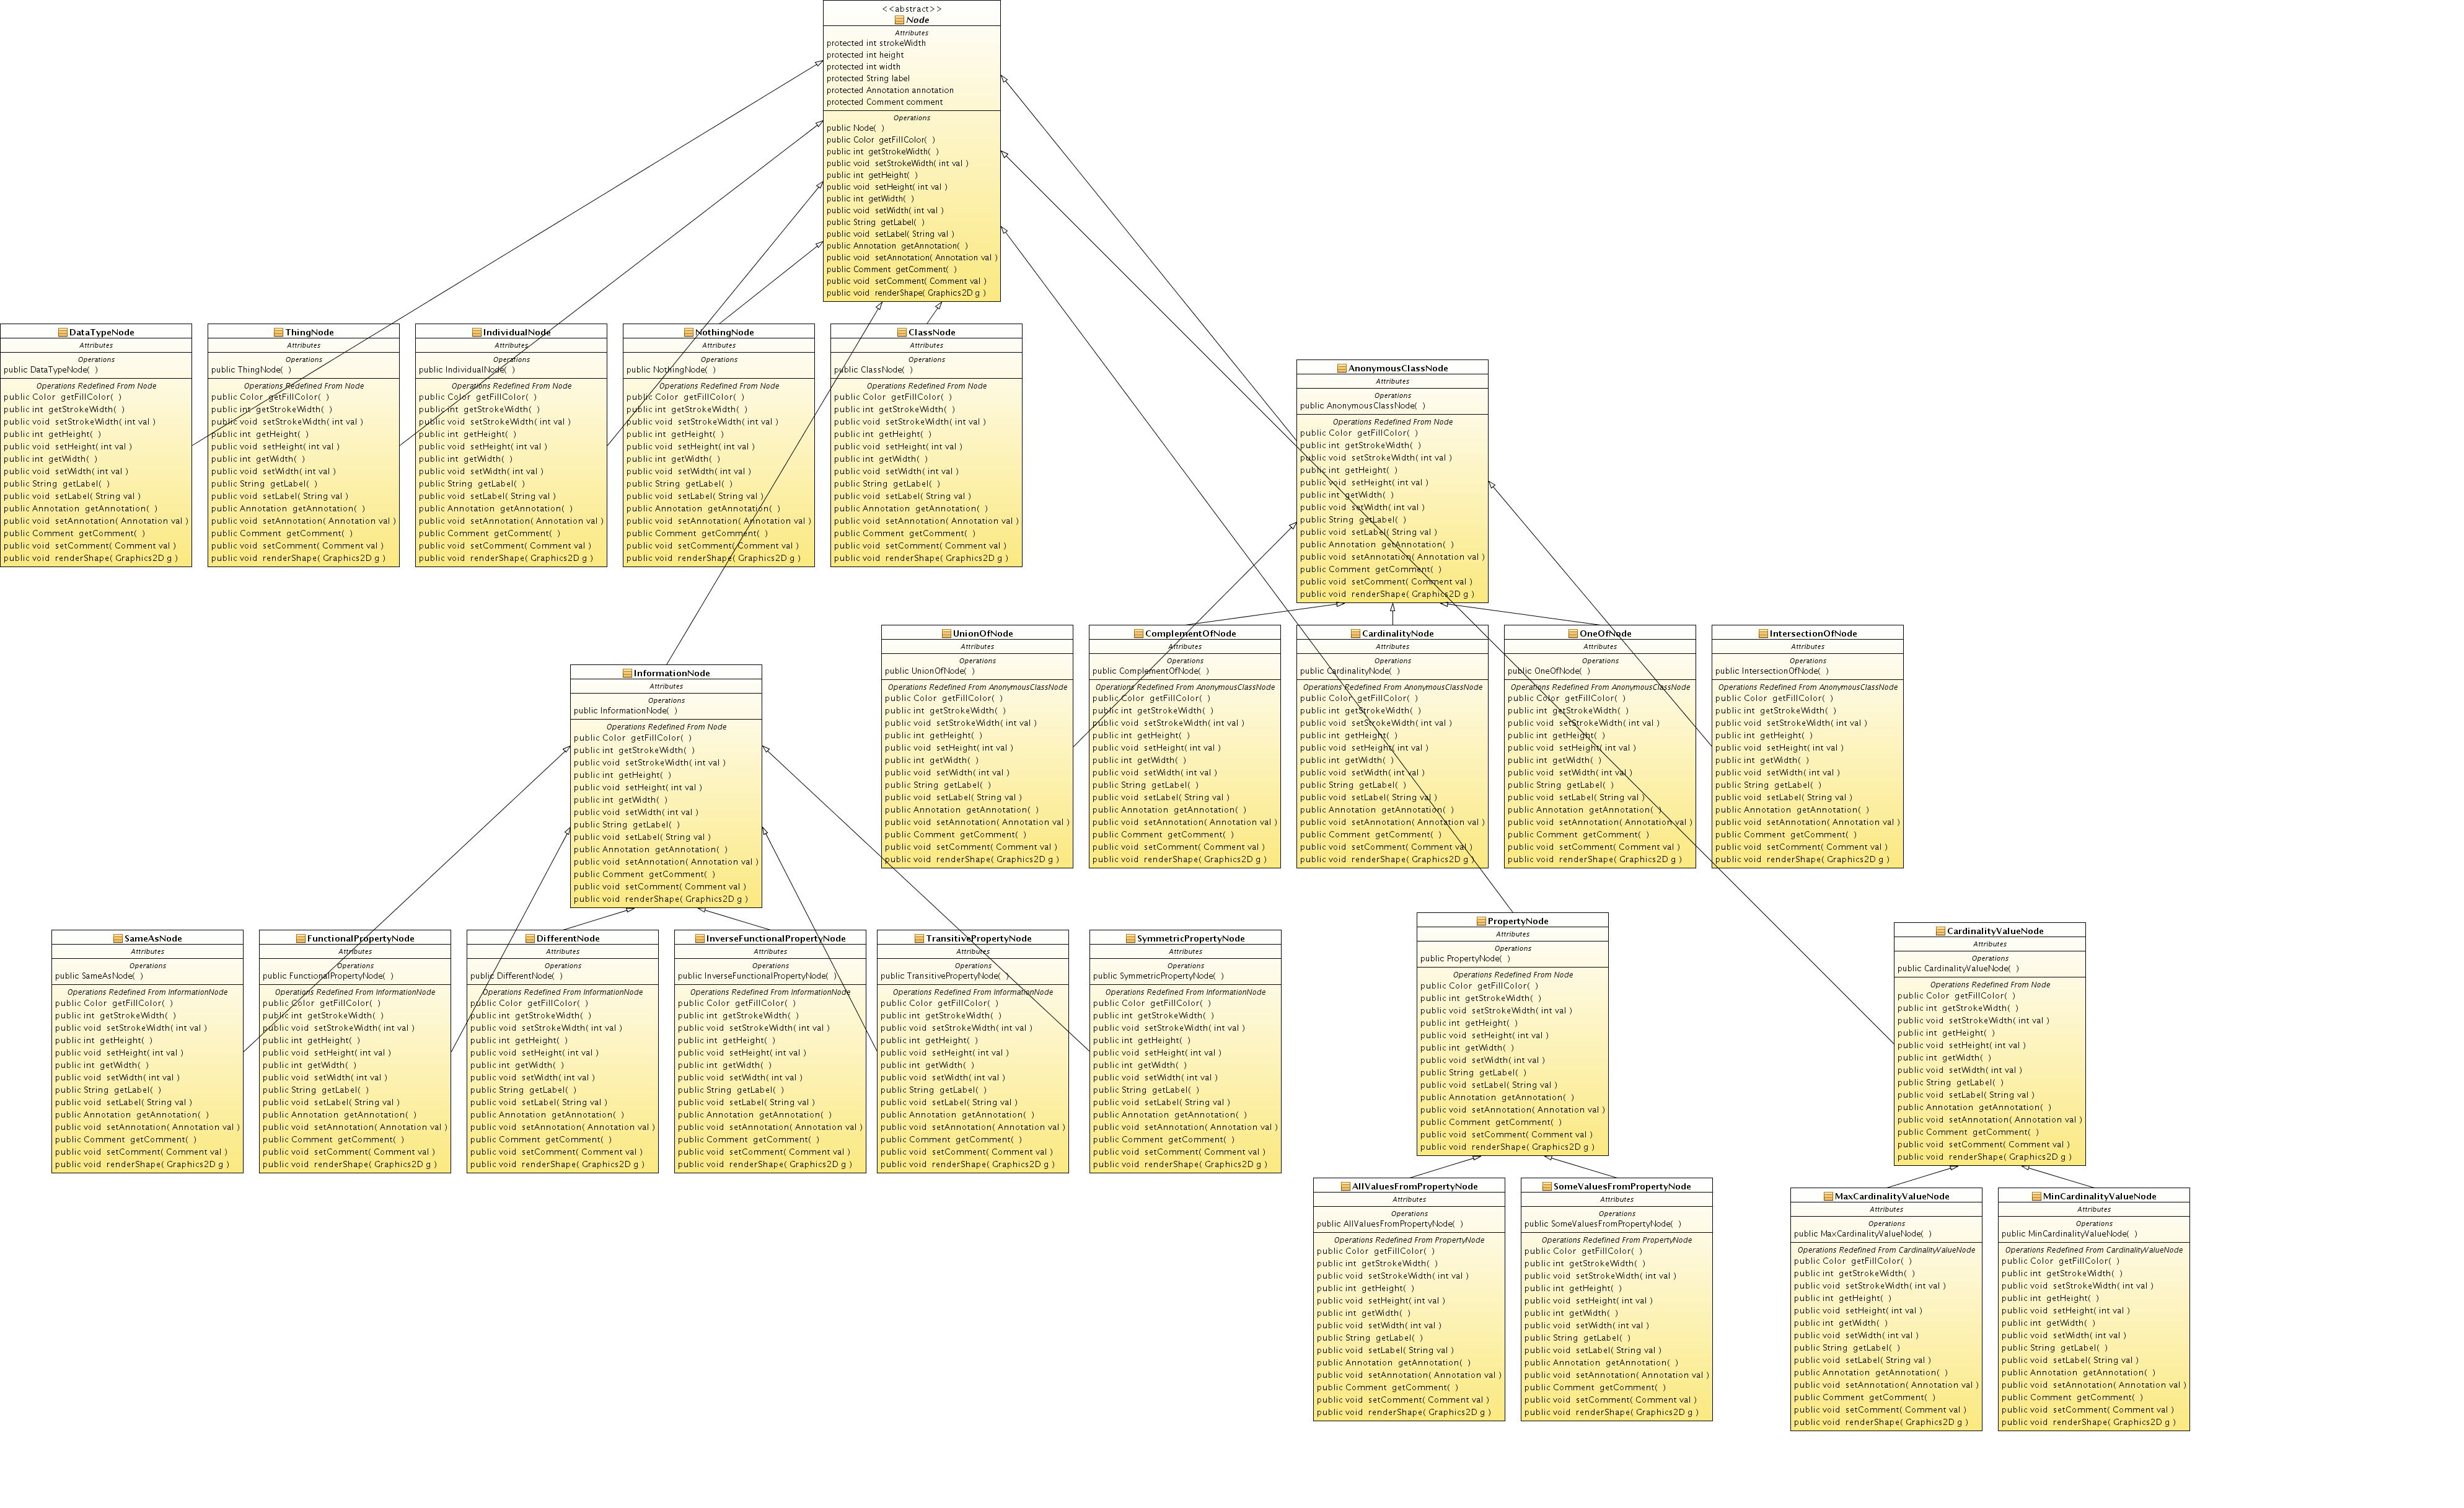
\includegraphics[width=\linewidth]{./modelowanie/OV_UML/NodesClassDiagram.png}}
\end{center}

\subsection{Opis klasy}

\begin{center}
 


\begin{longtable}{|m{3cm}|m{9cm}|} \hline

CN001 & Node \\ \hline
Opis: & Klasa nadrzędna względem wszystkich klas obsługi wierzchołków. Zawiera definicje podstawowych atrybutów i metod.    \\ \hline
Klasy nadrzędne: &     \\ \hline
Atrybuty: & \begin{itemize}
 \item strokeWidth
 \item label
\end{itemize}
 \\ \hline
Metody: & \begin{itemize}
 \item getFillColorFromScheme - zwraca kolor wypełnienia ustawiony dla tego węzła w zadanym schemacie
 \item getNodeShapeType - zwraca kształt węzła
\end{itemize}
  \\ \hline
Realizowane wymagania: & WF004, WF005, WF006, WF007, WI004 \\ \hline
Priorytet: & bardzo ważne  \\ \hline

\multicolumn{2}{c}{} \\
 \hline

CN002 & AllValuesFromPropertyNode \\ \hline
Opis: & Klasa reprezentuje wierzchołek, będący OWL Property typu AllValuesFrom.    \\ \hline
Klasy nadrzędne: & CN001 (Node)     \\ \hline
Atrybuty: & 
%\begin{itemize}
 %\item 
%\end{itemize}
 \\ \hline
Metody: & \begin{itemize}
 \item getFillColorFromScheme
 \item getNodeShapeType
\end{itemize}
  \\ \hline
Realizowane wymagania: & WF004, WF006, WF007, WI004 \\ \hline
Priorytet: & ważne \\ \hline

\multicolumn{2}{c}{} \\
 \hline

CN003 & AnonymousClassNode \\ \hline
Opis: & Klasa reprezentuje wierzchołek klas anonimowych OWL.    \\ \hline
Klasy nadrzędne: & CN001 (Node)       \\ \hline
Atrybuty: & \begin{itemize}
 \item anonymousId
\end{itemize}
 \\ \hline
Metody: & \begin{itemize}
 \item getFillColorFromScheme
\end{itemize}
  \\ \hline
Realizowane wymagania: & WF005, WI004 \\ \hline
Priorytet: & ważne \\ \hline

\multicolumn{2}{c}{} \\
 \hline

CN004 & CardinalityNode \\ \hline
Opis: & Klasa reprezentuje wierzchołek klas anonimowych OWL będących wynikiem ograniczenia kardynalności.    \\ \hline
Klasy nadrzędne: & CN003 (AnonymousNode)     \\ \hline
Atrybuty: & %\begin{itemize}
 %\item 
%\end{itemize}
 \\ \hline
Metody: & %\begin{itemize}
 %\item 
%\end{itemize}
  \\ \hline
Realizowane wymagania: & WF007, WI004 \\ \hline
Priorytet: & ważne  \\ \hline

\multicolumn{2}{c}{} \\
 \hline

CN005 & CardinalityValueNode \\ \hline
Opis: & Klasa reprezentuje wierzchołek z dokładnym ograniczeniem kardynalności (OWL Cardinality). \\ \hline
Klasy nadrzędne: & CN001 (Node)       \\ \hline
Atrybuty: & %\begin{itemize}
 %\item 
%\end{itemize}
 \\ \hline
Metody: & \begin{itemize}
 \item getFillColorFromScheme
 \item getNodeShapeType
\end{itemize}
  \\ \hline
Realizowane wymagania: & WF007, WI004 \\ \hline
Priorytet: & ważne  \\ \hline

\multicolumn{2}{c}{} \\
 \hline

CN006 & ClassNode \\ \hline
Opis: & Klasa reprezentuje wierzchołek OWL Class.    \\ \hline
Klasy nadrzędne: & CN001 (Node)       \\ \hline
Atrybuty: & %\begin{itemize}
 %\item 
%\end{itemize}
 \\ \hline
Metody: & \begin{itemize}
 \item getFillColorFromScheme
\end{itemize}
  \\ \hline
Realizowane wymagania: & WF004, WF005, WI004 \\ \hline
Priorytet: & ważne  \\ \hline

\multicolumn{2}{c}{} \\
 \hline

CN007 & ComplementOfNode \\ \hline
Opis: & Klasa reprezentuje wierzchołek klas anonimowych OWL będących wynikiem dopełnienia (OWL ComplementOf).    \\ \hline
Klasy nadrzędne: & CN001 (Node)       \\ \hline
Atrybuty: & %\begin{itemize}
 %\item 
%\end{itemize}
 \\ \hline
Metody: & %\begin{itemize}
 %\item 
%\end{itemize}
  \\ \hline
Realizowane wymagania: & WF006, WF007, WI004 \\ \hline
Priorytet: & ważne  \\ \hline

\multicolumn{2}{c}{} \\
 \hline

CN008 & DataTypeNode \\ \hline
Opis: & Klasa reprezentuje wierzchołek OWL DataType.    \\ \hline
Klasy nadrzędne: & CN001 (Node)       \\ \hline
Atrybuty: & %\begin{itemize}
 %\item 
%\end{itemize}
 \\ \hline
Metody: & \begin{itemize}
 \item getFillColorFromScheme
\end{itemize}
  \\ \hline
Realizowane wymagania: & WF004, WI04 \\ \hline
Priorytet: & ważne  \\ \hline

\multicolumn{2}{c}{} \\
 \hline

CN009 & DifferentNode \\ \hline
Opis: & Klasa reprezentuje wierzchołek oznaczający relację DifferentFrom lub AllDifferent pomiędzy wystąpieniami klas (OWL Individual).    \\ \hline
Klasy nadrzędne: & CN001 (Node)       \\ \hline
Atrybuty: & %\begin{itemize}
 %\item 
%\end{itemize}
 \\ \hline
Metody: & \begin{itemize}
 \item getFillColorFromScheme
\end{itemize}
  \\ \hline
Realizowane wymagania: & WF006, WF007, WI004 \\ \hline
Priorytet: & ważne  \\ \hline

\multicolumn{2}{c}{} \\
 \hline

CN010 & FunctionalPropertyNode \\ \hline
Opis: & Klasa reprezentuje wierzchołek oznaczający, że dane OWL Property to FunctionalProperty.  \\ \hline
Klasy nadrzędne: & CN010 (InformationNode)     \\ \hline
Atrybuty: & %\begin{itemize}
 %\item 
%\end{itemize}
 \\ \hline
Metody: & %\begin{itemize}
 %\item 
%\end{itemize}
  \\ \hline
Realizowane wymagania: & WF006, WF007, WI004 \\ \hline
Priorytet: & ważne  \\ \hline

\multicolumn{2}{c}{} \\
 \hline

CN011 & IndividualNode \\ \hline
Opis: & Klasa reprezentuje wierzchołek instancji OWL Individual.  \\ \hline
Klasy nadrzędne: & CN001 (Node)       \\ \hline
Atrybuty: & %\begin{itemize}
 %\item 
%\end{itemize}
 \\ \hline
Metody: & \begin{itemize}
 \item getFillColorFromScheme
 \item getNodeShapeType
\end{itemize}
  \\ \hline
Realizowane wymagania: & WF004, WI004 \\ \hline
Priorytet: & ważne  \\ \hline

\multicolumn{2}{c}{} \\
 \hline

CN012 & InformationNode \\ \hline
Opis: & Klasa ta jest klasą nadrzędną, dla klas wierzchołków reprezentujących informacje o różnych właściwościach OWL Property.    \\ \hline
Klasy nadrzędne: & CN001 (Node)       \\ \hline
Atrybuty: & %\begin{itemize}
 %\item 
%\end{itemize}
 \\ \hline
Metody: & \begin{itemize}
 \item getFillColorFromScheme
 \item getNodeShapeType
\end{itemize}
  \\ \hline
Realizowane wymagania: & WF010, WI004 \\ \hline
Priorytet: & ważne  \\ \hline

\multicolumn{2}{c}{} \\
 \hline

CN013 & IntersectionOfNode \\ \hline
Opis: & Klasa reprezentuje wierzchołek klas anonimowych OWL będących wynikiem przecięcia (OWL IntersectionOf).    \\ \hline
Klasy nadrzędne: & CN003 (AnonymousNode)     \\ \hline
Atrybuty: & %\begin{itemize}
 %\item 
%\end{itemize}
 \\ \hline
Metody: & %\begin{itemize}
 %\item 
%\end{itemize}
  \\ \hline
Realizowane wymagania: & WF005, WI004 \\ \hline
Priorytet: & ważne  \\ \hline

\multicolumn{2}{c}{} \\
 \hline

CN014 & InverseFunciotnalPropertyNode \\ \hline
Opis: & Klasa reprezentuje wierzchołek oznaczający, że dane OWL Property to InverseFunctionalProperty.    \\ \hline
Klasy nadrzędne: & CN010 (InformationNode)     \\ \hline
Atrybuty: & %\begin{itemize}
 %\item 
%\end{itemize}
 \\ \hline
Metody: & %\begin{itemize}
 %\item 
%\end{itemize}
  \\ \hline
Realizowane wymagania: & WF007, WI004 \\ \hline
Priorytet: & ważne  \\ \hline

\multicolumn{2}{c}{} \\
 \hline

CN015 & MaxCardinalityValueNode \\ \hline
Opis: & Klasa reprezentuje wierzchołek ograniczenia kardynalności OWL MaxCardinality.    \\ \hline
Klasy nadrzędne: & CN005 (CardinalityValueNode)     \\ \hline
Atrybuty: & %\begin{itemize}
 %\item 
%\end{itemize}
 \\ \hline
Metody: & \begin{itemize}
 \item getFillColorFromScheme
\end{itemize}
  \\ \hline
Realizowane wymagania: & WF007, WI004 \\ \hline
Priorytet: & ważne  \\ \hline

\multicolumn{2}{c}{} \\
 \hline

CN016 & MinCardinalityValueNode \\ \hline
Opis: & Klasa reprezentuje wierzchołek ograniczenia kardynalności OWL MinCardinality.    \\ \hline
Klasy nadrzędne: & CN005 (CardinalityValueNode)     \\ \hline
Atrybuty: & %\begin{itemize}
 %\item 
%\end{itemize}
 \\ \hline
Metody: & \begin{itemize}
 \item getFillColorFromScheme
\end{itemize}
  \\ \hline
Realizowane wymagania: & WF007, WI004 \\ \hline
Priorytet: & ważne  \\ \hline

\multicolumn{2}{c}{} \\
 \hline

CN017 & NothingNode \\ \hline
Opis: & Klasa reprezentuje wierzchołek OWL Nothing.    \\ \hline
Klasy nadrzędne: & CN001 (Node)       \\ \hline
Atrybuty: & %\begin{itemize}
 %\item 
%\end{itemize}
 \\ \hline
Metody: & \begin{itemize}
 \item getFillColorFromScheme
 \item getNodeShapeType
\end{itemize}
  \\ \hline
Realizowane wymagania: & WF004, WF005, WI004 \\ \hline
Priorytet: & ważne  \\ \hline

\multicolumn{2}{c}{} \\
 \hline

CN018 & OneOfNode \\ \hline
Opis: & Klasa reprezentuje wierzchołek klas anonimowych OWL reprezentujących 1 z klas określonego zbioru (wynik OWL OneOf).    \\ \hline
Klasy nadrzędne: & CN003 (AnonymousClassNode)     \\ \hline
Atrybuty: & %\begin{itemize}
 %\item 
%\end{itemize}
 \\ \hline
Metody: & %\begin{itemize}
 %\item 
%\end{itemize}
  \\ \hline
Realizowane wymagania: & WF005, WF006, WI004 \\ \hline
Priorytet: & ważne  \\ \hline

\multicolumn{2}{c}{} \\
 \hline

CN019 & PropertyNode \\ \hline
Opis: & Klasa reprezentuje wierzchołek OWL Property.    \\ \hline
Klasy nadrzędne: & CN001 (Node)       \\ \hline
Atrybuty: & %\begin{itemize}
 %\item 
%\end{itemize}
 \\ \hline
Metody: & \begin{itemize}
 \item getFillColorFromScheme
\end{itemize}
  \\ \hline
Realizowane wymagania: & WF004, WF007, WI004 \\ \hline
Priorytet: & ważne  \\ \hline

\multicolumn{2}{c}{} \\
 \hline

CN020 & SameAsNode \\ \hline
Opis: & Klasa reprezentuje wierzchołek oznaczający relację OWL SameAs pomiędzy wystąpieniami klas (OWL Individual).    \\ \hline
Klasy nadrzędne: & CN010 (InformationNode)     \\ \hline
Atrybuty: & %\begin{itemize}
 %\item 
%\end{itemize}
 \\ \hline
Metody: & \begin{itemize}
 \item getFillColorFromScheme
\end{itemize}
  \\ \hline
Realizowane wymagania: & WF005, WF006, WI004 \\ \hline
Priorytet: & ważne  \\ \hline

\multicolumn{2}{c}{} \\
 \hline

CN021 & SomeValuesFromPropertyNode \\ \hline
Opis: & Klasa reprezentuje wierzchołek, będący OWL Property typu SomeValuesFrom. \\ \hline
Klasy nadrzędne: & CN019 (PropertyNode) \\ \hline
Atrybuty: & %\begin{itemize}
 %\item 
%\end{itemize}
 \\ \hline
Metody: & \begin{itemize}
 \item getFillColorFromScheme
\end{itemize}
  \\ \hline
Realizowane wymagania: & WF005, WF006, WI004 \\ \hline
Priorytet: & ważne  \\ \hline

\multicolumn{2}{c}{} \\
 \hline

CN022 & SymmetricPropertNode \\ \hline
Opis: & Klasa reprezentuje wierzchołek oznaczający, że dane OWL Property to SymmetricProperty.    \\ \hline
Klasy nadrzędne: & CN010 (InformationNode)     \\ \hline
Atrybuty: & %\begin{itemize}
 %\item 
%\end{itemize}
 \\ \hline
Metody: & %\begin{itemize}
 %\item 
%\end{itemize}
  \\ \hline
Realizowane wymagania: & WF007, WI004 \\ \hline
Priorytet: & ważne  \\ \hline

\multicolumn{2}{c}{} \\
 \hline

CN023 & ThingNode \\ \hline
Opis: & Klasa reprezentuje wierzchołek OWL Thing.    \\ \hline
Klasy nadrzędne: & CN001 (Node)       \\ \hline
Atrybuty: & %\begin{itemize}
 %\item 
%\end{itemize}
 \\ \hline
Metody: & \begin{itemize}
 \item getFillColorFromScheme
 \item getNodeShapeType
\end{itemize}
  \\ \hline
Realizowane wymagania: & WF004, WF005, WI004 \\ \hline
Priorytet: & ważne  \\ \hline

\multicolumn{2}{c}{} \\
 \hline

CN024 & TreansitivePropertyNode \\ \hline
Opis: & Klasa reprezentuje wierzchołek oznaczający, że dane OWL Property to TransitiveProperty.    \\ \hline
Klasy nadrzędne: & CN010 (InformationNode)     \\ \hline
Atrybuty: & %\begin{itemize}
 %\item 
%\end{itemize}
 \\ \hline
Metody: & %\begin{itemize}
 %\item 
%\end{itemize}
  \\ \hline
Realizowane wymagania: & WF006, WF007, WI004 \\ \hline
Priorytet: & ważne  \\ \hline

\multicolumn{2}{c}{} \\
 \hline

CN025 & UnionOfNode \\ \hline
Opis: & Klasa reprezentuje wierzchołek klas anonimowych OWL będących wynikiem unii (OWL UnionOf).    \\ \hline
Klasy nadrzędne: & CN003 (AnonymousNode)     \\ \hline
Atrybuty: & %\begin{itemize}
 %\item 
%\end{itemize}
 \\ \hline
Metody: & %\begin{itemize}
 %\item 
%\end{itemize}
  \\ \hline
Realizowane wymagania: & WF005, WF006, WI004 \\ \hline
Priorytet: & ważne  \\ \hline

%\multicolumn{2}{c}{} \\
% \hline


\end{longtable}

\end{center}

\section{Pakiet edges}

\subsection{Diagram}

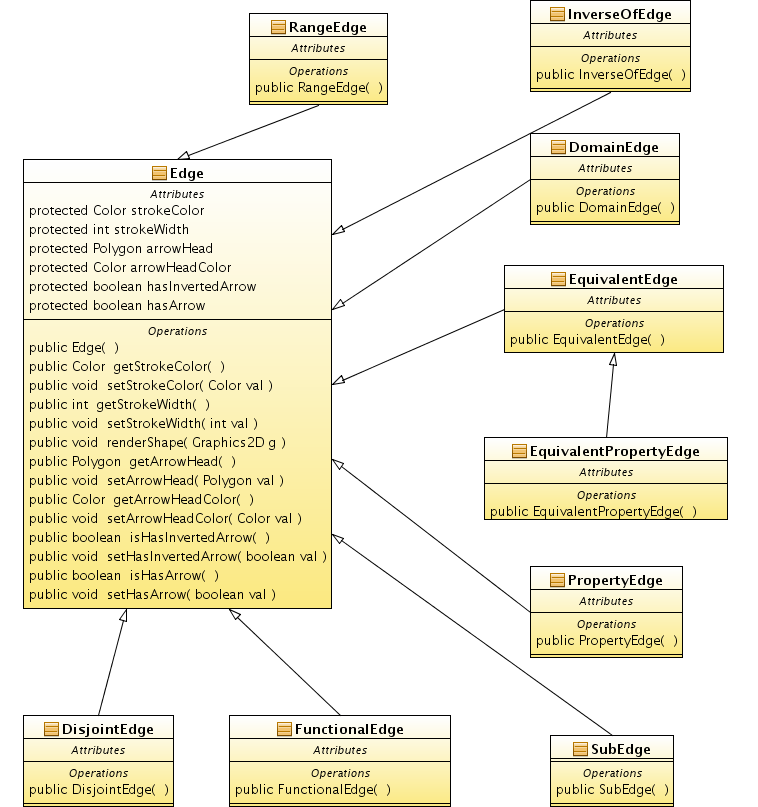
\includegraphics[width=\linewidth]{./modelowanie/OV_UML/EdgeClassDiagram.png} 

\subsection{Opis klasy}

\begin{center}

\begin{longtable}{|m{3cm}|m{9cm}|} \hline

CE001 & Edge \\ \hline
Opis: &  Klasa reprezentująca prostą krawędź na grafie. Jest nadklasą dla pozostałych klas krawędzi.  \\ \hline
Klasy nadrzędne: &     \\ \hline
Atrybuty: & \begin{itemize}
	\item boolean hasArrow
	\item boolean hasInvertedArrow
	\item Color arrowHeadColor
	\item Color strokeColor
	\item int strokeWidth 
\end{itemize}
 \\ \hline
Metody: & \begin{itemize}
	\item getStrokeColorFromScheme 
	\item getArrowHead
	\item getInvArrowHead
\end{itemize}
  \\ \hline
Realizowane wymagania: & WF006, WF007, WI004 \\ \hline
Priorytet: & bardzo ważne  \\ \hline

\multicolumn{2}{c}{} \\
 \hline

CE002 & DisjointEdge \\ \hline
Opis: & Klasa reprezentująca krawędź oznaczającą rozłączność klas (OWL Disjoint). \\ \hline
Klasy nadrzędne: & CE001 (Edge)    \\ \hline
Atrybuty: & %\begin{itemize}
 %\item 
%\end{itemize}
 \\ \hline
Metody: & \begin{itemize}
	\item getStrokeColorFromScheme
	\item getArrowHead
	\item getInvArrowHead
\end{itemize}
  \\ \hline
Realizowane wymagania: & WF006, WF007, WI004 \\ \hline
Priorytet: & ważne  \\ \hline

\multicolumn{2}{c}{} \\
 \hline

CE003 & DomainEdge  \\ \hline
Opis: & Klasa reprezentująca krawędź łączącą Property z klasą właściwości OWL DomainOf.   \\ \hline
Klasy nadrzędne: & CE001 (Edge) \\ \hline
Atrybuty: & %\begin{itemize}
 %\item 
%\end{itemize}
 \\ \hline
Metody: & \begin{itemize}
	\item getStrokeColorFromScheme
	\item getArrowHead
	\item getInvArrowHead
\end{itemize}
  \\ \hline
Realizowane wymagania: & WF006, WF007, WI004 \\ \hline
Priorytet: & ważne  \\ \hline

\multicolumn{2}{c}{} \\
 \hline

CE004 & EquivalentEdge \\ \hline
Opis: & Klasa reprezentująca krawędź oznaczającą równoznaczność (OWL Equivalent).    \\ \hline
Klasy nadrzędne: & CE001 (Edge)    \\ \hline
Atrybuty: & %\begin{itemize}
 %\item 
%\end{itemize}
 \\ \hline
Metody: & \begin{itemize}
	\item getStrokeColorFromScheme 
	\item getArrowHead
	\item getInvArrowHead
\end{itemize}
  \\ \hline
Realizowane wymagania: & WF006, WF007, WI004 \\ \hline
Priorytet: & ważne  \\ \hline

\multicolumn{2}{c}{} \\
 \hline

CE005 & EquivalentPropertyEdge \\ \hline
Opis: & Klasa reprezentująca krawędź oznaczającą równoznaczność OWL Property (OWL EquivalentProperty).    \\ \hline
Klasy nadrzędne: & CE004 (EquivalentEdge)    \\ \hline
Atrybuty: & %\begin{itemize}
 %\item 
%\end{itemize}
 \\ \hline
Metody: & \begin{itemize}
	\item getStrokeColorFromScheme
\end{itemize}
  \\ \hline
Realizowane wymagania: & WF006, WF007, WI004 \\ \hline
Priorytet: & ważne  \\ \hline

\multicolumn{2}{c}{} \\
 \hline

CE006 & FunctionaltEdge \\ \hline
Opis: & Klasa reprezentująca krawędź łączącą wierzchołki InformationNode(CN012) z OWL Property, którego dotyczy.   \\ \hline
Klasy nadrzędne: & CE001 (Edge)    \\ \hline
Atrybuty: & %\begin{itemize}
 %\item 
%\end{itemize}
 \\ \hline
Metody: & \begin{itemize}
	\item getStrokeColorFromScheme
\end{itemize}
  \\ \hline
Realizowane wymagania: & WF006, WF007, WI004 \\ \hline
Priorytet: & ważne  \\ \hline

\multicolumn{2}{c}{} \\
 \hline

CE007 & InverseOfEdge \\ \hline
Opis: & Klasa reprezentująca krawędź oznaczającą odwrotność (OWL InverseOf).    \\ \hline
Klasy nadrzędne: & CE001 (Edge)    \\ \hline
Atrybuty: & %\begin{itemize}
 %\item 
%\end{itemize}
 \\ \hline
Metody: & \begin{itemize}
	\item getStrokeColorFromScheme 
	\item getArrowHead
	\item getInvArrowHead
\end{itemize}
  \\ \hline
Realizowane wymagania: & WF006, WF007, WI004 \\ \hline
Priorytet: & ważne  \\ \hline

\multicolumn{2}{c}{} \\
 \hline

CE008 & PropertyEdge \\ \hline
Opis: &  Klasa reprezentująca krawędź oznaczającą relację między Property a klasą.   \\ \hline
Klasy nadrzędne: & CE001 (Edge)    \\ \hline
Atrybuty: & %\begin{itemize}
 %\item 
%\end{itemize}
 \\ \hline
Metody: & \begin{itemize}
	\item getStrokeColorFromScheme 
	\item getArrowHead
	\item getInvArrowHead
\end{itemize}
  \\ \hline
Realizowane wymagania: & WF006, WF007, WI004 \\ \hline
Priorytet: & ważne  \\ \hline

\multicolumn{2}{c}{} \\
 \hline

CE009 & RangeEdge \\ \hline
Opis: & Klasa reprezentująca na grafie krawędź łączącą Property z klasą właściwości OWL Range.     \\ \hline
Klasy nadrzędne: & CE001 (Edge)    \\ \hline
Atrybuty: & %\begin{itemize}
 %\item 
%\end{itemize}
 \\ \hline
Metody: & \begin{itemize}
	\item getStrokeColorFromScheme 
	\item getArrowHead
	\item getInvArrowHead
\end{itemize}
  \\ \hline
Realizowane wymagania: & WF006, WF007, WI004 \\ \hline
Priorytet: & ważne  \\ \hline

\multicolumn{2}{c}{} \\
 \hline

CE010 & SubEdge \\ \hline
Opis: & Klasa reprezentująca krawędź związku OWL SubClass pomiędzy klasami.   \\ \hline
Klasy nadrzędne: & CE001 (Edge)    \\ \hline
Atrybuty: & %\begin{itemize}
 %\item 
%\end{itemize}
 \\ \hline
Metody: & \begin{itemize}
	\item getInvArrowHead
\end{itemize}
  \\ \hline
Realizowane wymagania: & WF006, WF007, WI004 \\ \hline
Priorytet: & ważne  \\ \hline

\multicolumn{2}{c}{} \\
 \hline

CE011 & InverseOfMutualEdge \\ \hline
Opis: & Klasa reprezentująca krawędź oznaczającą wzajemną odwrotność (OWL InverseOf) property. \\ \hline
Klasy nadrzędne: & CE007 (InverseOfEdge)    \\ \hline
Atrybuty: & %\begin{itemize}
 %\item 
%\end{itemize}
 \\ \hline
Metody: & 
  \\ \hline
Realizowane wymagania: & WF006, WF007, WI004 \\ \hline
Priorytet: & ważne  \\ \hline

\multicolumn{2}{c}{} \\
 \hline

CE012 & OperationEdge \\ \hline
Opis: & Krawędź do oznaczania powiązań operacji, w wyniku których powstają klasy anonimowe. \\ \hline
Klasy nadrzędne: & CE001 (Edge)    \\ \hline
Atrybuty: & %\begin{itemize}
 %\item 
%\end{itemize}
 \\ \hline
Metody: & \begin{itemize}
	\item getArrowHead
\end{itemize} 
  \\ \hline
Realizowane wymagania: & WF006, WF007, WI004 \\ \hline
Priorytet: & ważne  \\ \hline


%\multicolumn{2}{c}{} \\
% \hline


\end{longtable}

\end{center}

\section{Pakiet visualization }

\subsection{Diagram}

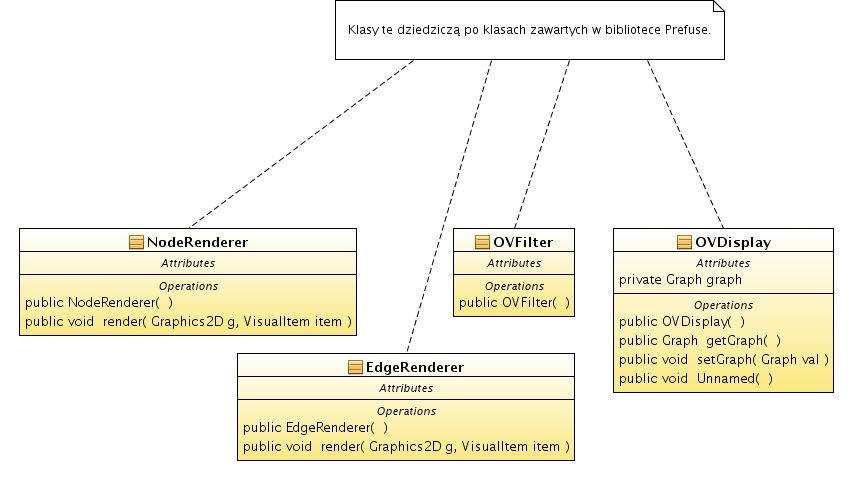
\includegraphics[width=\linewidth]{./modelowanie/OV_UML/VisualizationClassDiagram.png}

\subsection{Opis klasy}

\begin{center}
 

\begin{longtable}{|m{3cm}|m{9cm}|} \hline

CV001 & EdgeRenderer \\ \hline
Opis: & Klasa przeciążająca metody renderowania krawędzi grafu z biblioteki prefuse. \\ \hline
Klasy nadrzędne: &  prefuse.render.EdgeRenderer   \\ \hline
Atrybuty: & %\begin{itemize}
 %\item 
%\end{itemize}
 \\ \hline
Metody: & \begin{itemize}
	\item render(Graphics2D g, VisualItem item) - metoda renderująca krawędź	
\end{itemize}
  \\ \hline
Realizowane wymagania: & WF001, WF008, WI004 \\ \hline
Priorytet: & ważne  \\ \hline

\multicolumn{2}{c}{} \\
 \hline

CV002 & NodeRenderer \\ \hline
Opis: & Klasa przeciążająca metody renderowania wierzchołków grafu z biblioteki prefuse.    \\ \hline
Klasy nadrzędne: &  prefuse.render.LabelRenderer   \\ \hline
Atrybuty: & %\begin{itemize}
 %\item 
%\end{itemize}
 \\ \hline
Metody: & \begin{itemize}
	\item drawString(Graphics2D g, FontMetrics fm, String text,
            boolean useInt, double x, double y, double w) - metoda wypisujaca na wierzchołku String
	\item render (Graphics2D g, VisualItem item) - metoda renderująca wierzchołek
	\item Shape changeShapeToCircle(Shape rectangleShape) - Zamienia domyślny, prostokątny kształt węzła na koło. Koło to ma średnicę równą szerokości lub wysokości węzła (większa z wartości) i środek w tym samym punkcie.
\end{itemize}
  \\ \hline
Realizowane wymagania: & WF001, WF008, WI004 \\ \hline
Priorytet: & ważne  \\ \hline

\multicolumn{2}{c}{} \\
 \hline

CV003 & OVDisplay \\ \hline
Opis: &  Klasa tworząca obiekt JComponent do umieszczenia na okienku JAVA zawierający wygenerowany graf z wizualizacją   \\ \hline
Klasy nadrzędne: &  prefuse.Display   \\ \hline
Atrybuty: & \begin{itemize}
 \item Graph graph - obiekt typu prefuse.data.graph zawierajacy dane o grafie do wyświetlenia. 
\end{itemize}
 \\ \hline
Metody: & \begin{itemize}
	\item generateGraphFromOWl(OWLOntology ont) - wpisuje do klasy obiekt Grpah wygenrowany na podstawie ontologii
	\item refreshVisualization()
\end{itemize}
  \\ \hline
Realizowane wymagania: & WF001, WF002, WF008, WI004 \\ \hline
Priorytet: & ważne  \\ \hline

% \multicolumn{2}{c}{} \\
%  \hline
% 
% CV004 & OVFilter \\ \hline
% Opis: & Klasa zawierająca filtry służace do wyświetlania danych w różnych zakresach    \\ \hline
% Klasy nadrzędne: &     \\ \hline
% Atrybuty: & %\begin{itemize}
%  %\item 
% %\end{itemize}
%  \\ \hline
% Metody: & %\begin{itemize}
%  %\item 
% %\end{itemize}
%   \\ \hline
% Realizowane wymagania: & WF001, WF008, WI004 \\ \hline
% Priorytet: & ważne  \\ \hline

\multicolumn{2}{c}{} \\
 \hline

CV005 & ForceDirectedVis \\ \hline
Opis: &  Klasa wizualizujące grafy w oparciu o algorytm ForceDirected   \\ \hline
Klasy nadrzędne: & CV007 (OVVisualization)   \\ \hline
Atrybuty: & 
 \\ \hline
Metody: & 
  \\ \hline
Realizowane wymagania: & WF001, WF002, WF008, WI004 \\ \hline
Priorytet: & ważne  \\ \hline

\multicolumn{2}{c}{} \\
 \hline

CV006 & OVPredicate \\ \hline
Opis: &  Klasa zawierająca predykaty filtrowania obiektów w wyswietlanych grafach \\ \hline
Klasy nadrzędne: &  prefuse.data.expression.AbstractPredicate   \\ \hline
Atrybuty: & \begin{itemize}
	\item boolean disjointEdgeFilter
	\item boolean subEdgeFilter
\end{itemize}
 \\ \hline
Metody: & %\begin{itemize}
	%\item generateGraphFromOWl(OWLOntology ont) - wpisuje do klasy obiekt Grpah wygenrowany na podstawie ontologii
	%\item refreshVisualization()
%\end{itemize}
  \\ \hline
Realizowane wymagania: & WF001, WF002, WF008, WI004 \\ \hline
Priorytet: & ważne  \\ \hline

\multicolumn{2}{c}{} \\
 \hline

CV007 & OVVisualization \\ \hline
Opis: &  Klasa obsługi wizualizacji. \\ \hline
Klasy nadrzędne: &  prefuse.Visualization   \\ \hline
Atrybuty: & 
 \\ \hline
Metody: & \begin{itemize}
	\item refreshFilter()
	\item startLayout()
	\item stopLayout()
\end{itemize}
  \\ \hline
Realizowane wymagania: & WF001, WF002, WF008, WI004 \\ \hline
Priorytet: & ważne  \\ \hline

\multicolumn{2}{c}{} \\
 \hline

CV008 & RadialGraphVis \\ \hline
Opis: &  Klasa wizualizująca graf w oparciu o algorytm RadialGraph \\ \hline
Klasy nadrzędne: &  CV007 (OVVisualization)   \\ \hline
Atrybuty: & 
 \\ \hline
Metody: & % \begin{itemize}
% 	\item refreshFilter()
% 	\item startLayout()
% 	\item stopLayout()
% \end{itemize}
  \\ \hline
Realizowane wymagania: & WF001, WF002, WF008, WI004 \\ \hline
Priorytet: & średnio ważne  \\ \hline

%\multicolumn{2}{c}{} \\
% \hline


\end{longtable}

\end{center}

\section{Pakiet graph}

\subsection{Diagram}

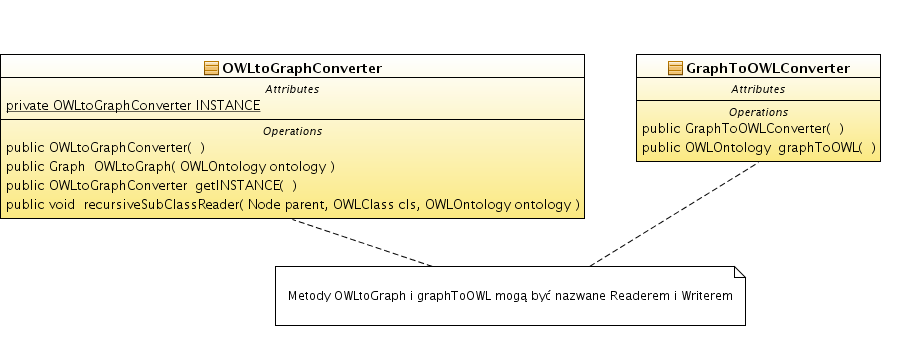
\includegraphics[width=\linewidth]{./modelowanie/OV_UML/GraphClassDiagram.png}

\subsection{Opis klasy}

\begin{center}
 


\begin{longtable}{|m{3cm}|m{9cm}|} \hline

CG001 & GraphToOWLConverter \\ \hline
Opis: & Klasa zawierająca metody pozwalające na przetwarzanie obiektów grafów z prefuse na obiekty OWL API. Klasa jest singletonem. \\ \hline
Klasy nadrzędne: &     \\ \hline
Atrybuty: & \begin{itemize}
 \item INSTANCE - instancja klasy GraphToOWLConverter 
\end{itemize}
 \\ \hline
Metody: & \begin{itemize}
	\item getInstance() - zwraca instancję klasy
	\item GraphToOWL(OWLOntology ontology) -Zamienia graf z biblioteki prefuse na ontologię zapisana w OWL API.
\end{itemize}
  \\ \hline
Realizowane wymagania: & WD001, WI004 \\ \hline
Priorytet: & ważne  \\ \hline

\multicolumn{2}{c}{} \\
 \hline

CG002 & OWLtoGraphConverter \\ \hline
Opis: & Klasa zawierająca metody pozwalające na przetwarzanie obiektów OWL API na obiekty prefuse. Klasa jest singletonem.\\ \hline
Klasy nadrzędne: &     \\ \hline
Atrybuty: & \begin{itemize}
	\item INSTANCE - instancja klasy GraphToOWLConverter 
	\item Table edges
	\item Table nodes
\end{itemize}
 \\ \hline
Metody: & \begin{itemize}
	\item getInstance() - zwraca instancję klasy
	\item insertAnonymousNodesAndEdges(OWLOntology ontology,  Graph graph,  Hashtable properties, Hashtable classes, Hashtable individuals)
	\item insertBaseClasses(OWLOntology ontology,  Graph graph, Node thing, Hashtable classes )
	\item insertBaseProperties(OWLOntology ontology,  Graph graph,  Hashtable properties)
	\item insertBaseIndividuals(OWLOntology ontology,  Graph graph,  Hashtable individuals)
	\item insertBasicEdgesForIndividuals(OWLOntology ontology,  Graph graph, Hashtable individuals,Hashtable classes )
	\item insertBasicEdgesForClasses(OWLOntology ontology,  Graph graph, Hashtable classes)
	\item insertBasicEdgesForProperties(OWLOntology ontology,  Graph graph,  Hashtable properties, Hashtable classes)
	
	%\item recursiveSubClassReader(Node parent, OWLClass cls,OWLOntology ontology ) - wczytuje do grafu OWL wszystkie klasy wraz z ich podklasami.
 	\item OWLToGraph(OWLOntology ontology) -Zamienia ontologię w OWL API na graf z biblioteki prefuse.
\end{itemize}
  \\ \hline
Realizowane wymagania: & WD001, WI004 \\ \hline
Priorytet: & ważne  \\ \hline

%\multicolumn{2}{c}{} \\
% \hline


\end{longtable}

\end{center}



\section{Pakiet utils}

\subsection{Diagram}

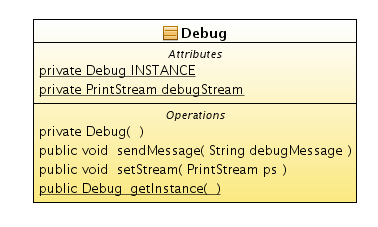
\includegraphics[width=\linewidth]{./modelowanie/OV_UML/UtilsDiagram.png}

\subsection{Opis klasy}

\begin{center}

\begin{tabular}{|m{3cm}|m{9cm}|} \hline

CU001 & Debug \\ \hline
Opis: & Klasa do użycia przy debugowaniu, zapewnia strumien z błędami zwracanymi przez bibliotekę. Klasa jest singletonem.\\ \hline
Klasy nadrzędne: &     \\ \hline
Atrybuty: & \begin{itemize}
 \item INSTANCE - instacja klasy Debug
 \item debugStream - Strumień do którego wpisywane są informacje potrzebne do debugowania
\end{itemize}
 \\ \hline
Metody: & \begin{itemize}
 \item getInstance() - zwraca instację klasy
 \item setStream(PrintStream ps) - ustawia podany strumień jako strumień na który zwracane będa błędy
 \item sendMessage(String s) - wysyła wiadomość na strumień do debugowania, jeżeli został wcześniej podpięty za pomocą funkcji setStream 	
\end{itemize}
  \\ \hline
Realizowane wymagania: & WF006, WF007, WI004 \\ \hline
Priorytet: & bardzo ważne  \\ \hline

\multicolumn{2}{c}{} \\
 \hline
 
CU002 & VisualizationProperties \\ \hline
Opis: & Klasa odpowiada za wczytywanie ustawień kolorów dla węzłów oraz krawędzi z wybranego lub domyślnego. \\ \hline
Klasy nadrzędne: &     \\ \hline
Atrybuty: & \begin{itemize}
 \item properties
\end{itemize}
 \\ \hline
Metody: & \begin{itemize}
 \item loadProperties
 \end{itemize}
  \\ \hline
Realizowane wymagania: & WF002 \\ \hline
Priorytet: & ważne  \\ \hline 
 
\end{tabular}
\end{center}

%\clearpage
%\phantomsection
%\addcontentsline{toc}{section}{Literatura}
%\bibliography{biblio}

\end{document}
